\documentclass{beamer}


%%% EU logo
% small version for upper right corner of normal pages
\pgfdeclareimage[width=12.8cm]{university-logo}{JRC_header}
\logo{\pgfuseimage{university-logo}}
\pgfdeclareimage[height=5.5mm]{footimage}{JRC_footer}
\newcommand{\titleimage}[1]{\pgfdeclareimage[width=0.5\textwidth]{title-image}{#1}}
%\newcommand{\footimage}{\pgfdeclareimage[width=0.5\textwidth]{title-image}{#1}}
\titlegraphic{\pgfuseimage{title-image}}
%%% end EU logo

% NOTE: 1cm = 0.393 in = 28.346 pt;    1 pt = 1/72 in = 0.0352 cm
\setbeamersize{text margin right=3.5mm, text margin left=7.5mm}  % text margin

% colors to be used
\definecolor{text-grey}{rgb}{0.45, 0.45, 0.45} % grey text on white background
\definecolor{bg-grey}{rgb}{0.66, 0.65, 0.60} % grey background (for white text)
\definecolor{eu-blue}{RGB}{55, 172, 222} % blue text
\definecolor{drk-blue}{RGB}{0, 51, 102} % blue text
\definecolor{fu-blue}{RGB}{0, 51, 102} % blue text
\definecolor{fu-green}{RGB}{153, 204, 0} % green text
\definecolor{fu-red}{RGB}{204, 0, 0} % red text (used by \alert)

% switch off the sidebars
\setbeamersize{sidebar width left=0cm, sidebar width right=0mm}
\setbeamertemplate{sidebar right}{}
\setbeamertemplate{sidebar left}{}
\setbeamertemplate{navigation symbols}{}%remove navigation symbols

% frame title
\setbeamertemplate{frametitle}{%
    \vskip-5pt \color{drk-blue}\Large%
    \begin{minipage}[b][23pt]{\textwidth}%
    \flushleft \textbf{\insertframetitle}%
    \end{minipage}%
}

%%% title page
\setbeamertemplate{title page}{

% set the title
\parbox[top][2.8cm][c]{\textwidth}{\begin{center} \color{drk-blue}\LARGE \textbf{\inserttitle}  \\ \vspace{10pt} \small \insertsubtitle \end{center}}

% title image of the presentation
\begin{minipage}{0.5\textwidth}
\flushleft
%\hspace{-7.5mm}
\inserttitlegraphic
\end{minipage}
% Author info
\hspace{0.5cm}
\begin{minipage}{0.4\textwidth}
{\flushleft \color{black} \textbf{\insertauthor} \\ \insertinstitute }
\end{minipage}
}
%%% end title page

%%% colors
\usecolortheme{lily}
\setbeamercolor*{normal text}{fg=drk-blue, bg=white}
\setbeamercolor*{alerted text}{fg=fu-red}
\setbeamercolor*{example text}{fg=fu-green}
\setbeamercolor*{structure}{fg=fu-blue}

\setbeamercolor*{block title}{fg=white,bg=black!50}
\setbeamercolor*{block title alerted}{fg=white,bg=black!50}
\setbeamercolor*{block title example}{fg=white,bg=black!50}

\setbeamercolor*{block body}{bg=black!10}
\setbeamercolor*{block body alerted}{bg=black!10}
\setbeamercolor*{block body example}{bg=black!10}

\setbeamercolor{item}{fg=eu-blue}
%%% end colors

\setbeamertemplate{itemize items}[circle] % if you want a ball
\setbeamertemplate{itemize subitem}[circle] % if you wnat a circle
\setbeamertemplate{itemize subsubitem}[cirlce] % if you want a triangle

%%% headline
\setbeamertemplate{headline}{
\insertlogo % logo on the right
%\begin{center}
%\colorbox{eu-blue}{
% \begin{minipage}[t]{.8\textwidth} \color{eu-blue} text \vspace{25pt} %\end{minipage}}
%\begin{minipage}[c]{0.0\textwidth}
%\hspace{-10mm} hi
%\end{minipage}
%\end{center}
}
%%% end headline

%%% footline
\newcommand{\footlinetext}{\insertdate}
\setbeamertemplate{footline}{
\begin{minipage}{58mm}
 \color{drk-blue} \hspace{7.5mm} \footlinetext
\end{minipage}
\hspace{0.1mm} 
\begin{minipage}{8.5mm}
 \pgfuseimage{footimage}
\end{minipage}
\hspace{0.1mm}
\begin{minipage}{50mm}
 \color{drk-blue} 
 %\raisebox{-1pt}{\usebeamertemplate***{navigation symbols}}
 \flushright \insertframenumber
\end{minipage}

}
%%% end footline
 
\usepackage{arev,t1enc}
\usepackage{amsmath}

\usepackage[T1]{fontenc}
\fontfamily{verdana}\selectfont

\title{The Costs of Ignoring Stock Structure}
%\subtitle{}
\author{Colin Millar\\Ernesto Jardim\\Iago Mosqueira\\Chato Osio}
\institute{European Commission\\ Joint Research Center}
\subject{Fisheries Management}

\usepackage{Sweave}
\begin{document}
\setkeys{Gin}{width=1.1\textwidth}

%% set up R environment
%<<echo=FALSE, results=hide>>=
%library(RColorBrewer)
%library(lattice)
%library(xtable)
%library(Hmisc)
%load("../presentation-data.rda")
%@

%%%%%%%%%%%%%%%%%%%%%%%%%%%%%%%%%%%%%%%%%%%%%

\begin{frame}
\titlepage
\end{frame}

%%%%%%%%%%%%%%%%%%%%%%%%%%%%%%%%%%%%%%%%%%%%%

\begin{withoutheadline}
\begin{frame}{Motivation}

  \begin{itemize}
    \item By:
    \begin{itemize}
      \item Simulating a range of realistic stock dynamics
      \item Modelling fisheries management
    \end{itemize}
    \item We aim to:
    \begin{itemize}
      \item Investigate managing two stocks as one
      \item Identify risks
      \item Suggest robust reference points
    \end{itemize}
  \end{itemize}
\end{frame}
\end{withoutheadline}

%%%%%%%%%%%%%%%%%%%%%%%%%%%%%%%%%%%%%%%%%%%%%

\begin{withoutheadline}
\begin{frame}{assessment 4 all - a4a}
  Some notes on a4a  
\end{frame}
\end{withoutheadline}

%%%%%%%%%%%%%%%%%%%%%%%%%%%%%%%%%%%%%%%%%%%%%

\begin{withoutheadline}
\begin{frame}{Simulation Design}
  The Population Model
  \begin{figure}
    \centering
    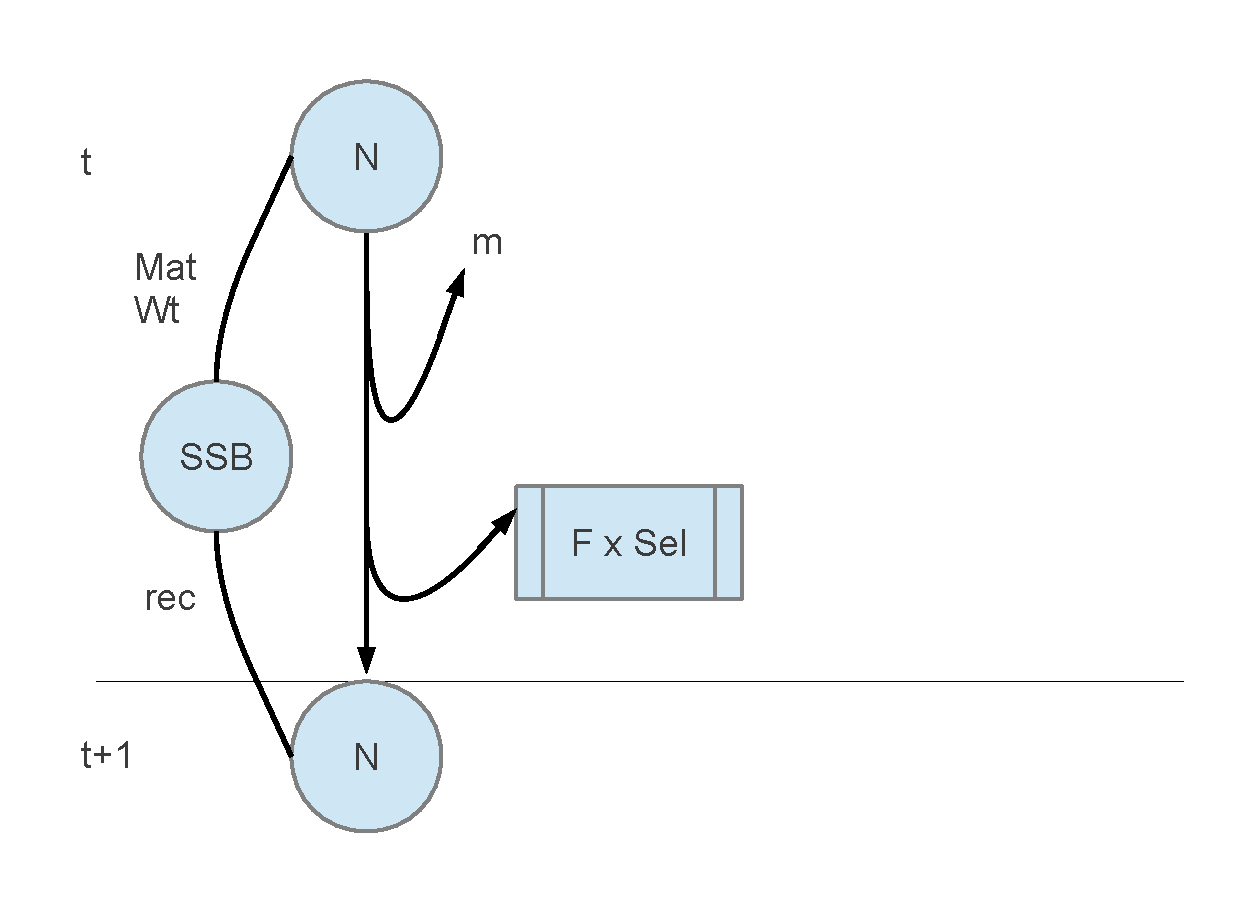
\includegraphics[width=.9\textwidth]{Population-model-half}
  \end{figure}
\end{frame}
\end{withoutheadline}


\begin{withoutheadline}
\begin{frame}{Simulation Design}
  The Population Model
  \begin{figure}
    \centering
    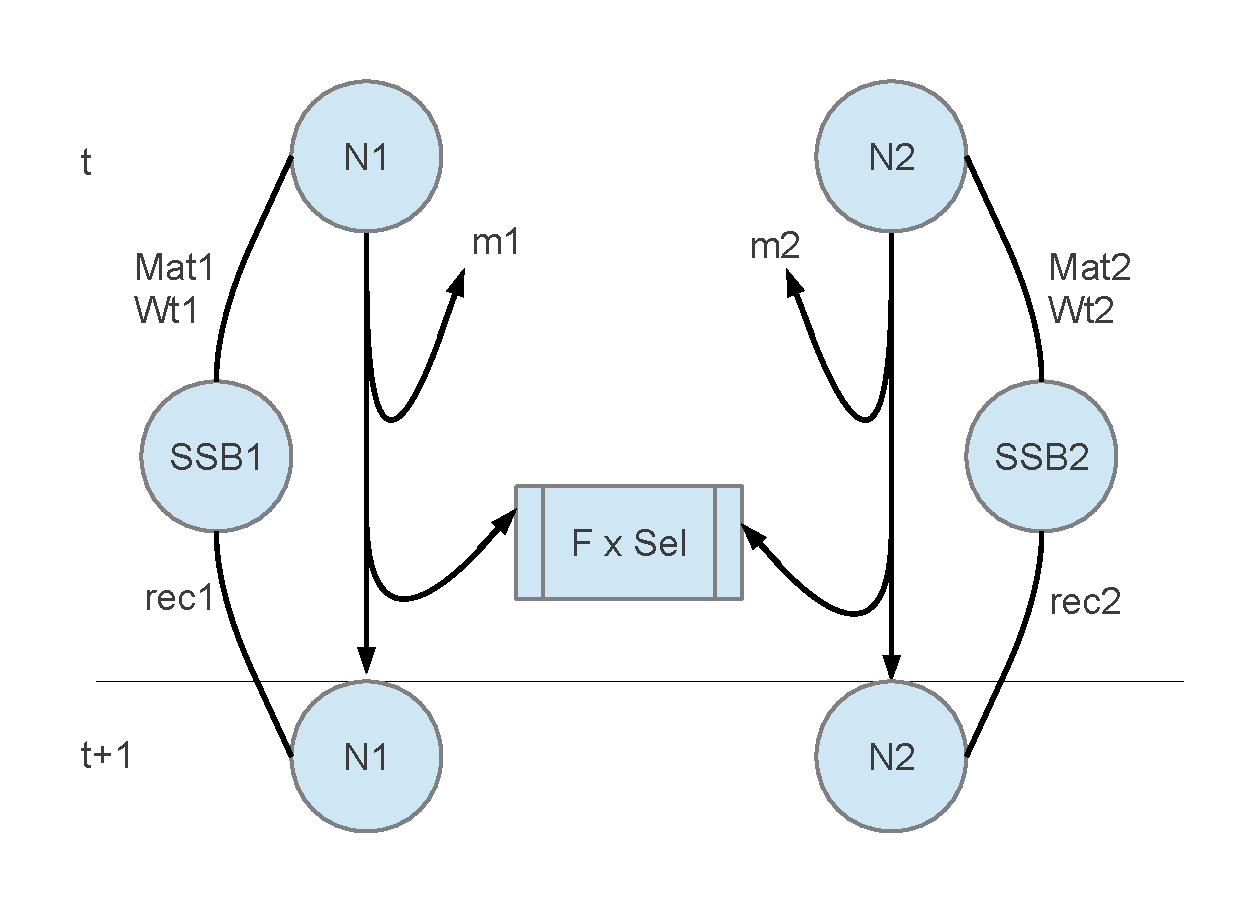
\includegraphics[width=.9\textwidth]{Population-model}
  \end{figure}
\end{frame}
\end{withoutheadline}

\begin{withoutheadline}
\begin{frame}{Simulation Design}
  The Population Model: candidate model for
  \begin{itemize}
    \item Lophius Piscatorius and Budagassa
    \item Atlantic Blue-Fin Tuna
    \item Whitining in the North Sea...?
  \end{itemize}
\end{frame}
\end{withoutheadline}



%%%%%%%%%%%%%%%%%%%%%%%%%%%%%%%%%%%%%%%%%%%%%


\begin{withoutheadline}
\begin{frame}{Simulation Design}
  Assessment inputs:
  \begin{align*}
    \text{Observed log Catch} &\sim \text{Normal}(\log \text{Catch}, 0.1) \\
    \text{Observed log Index} &\sim \text{Normal}(\log \text{Index}, 0.1)
  \end{align*}
  \begin{minipage}{0.4\textwidth}
  \begin{align*}
    \text{Catch} &= \text{Catch}_1 + \text{Catch}_2 \\
    \text{Index} &= q \times (N_1 + N_2)
  \end{align*}
  \end{minipage}
  \begin{minipage}{0.4\textwidth}
  \begin{align*}
    M &= 0.5 (M_1 + M_2) \\
    \text{Mat} &= 0.5 (\text{Mat}_1 + \text{Mat}_2) \\
    \text{wt} &= \frac{N_1 \text{wt}_1 + N_2 \text{wt}_2 }{N_1 + N_2}
  \end{align*}
  \end{minipage}
\end{frame}
\end{withoutheadline}

%%%%%%%%%%%%%%%%%%%%%%%%%%%%%%%%%%%%%%%%%%%%%
\begin{withoutheadline}
\begin{frame}{Simulation Design}
  Assessment Model and Management procedure
\end{frame}
\end{withoutheadline}

%%%%%%%%%%%%%%%%%%%%%%%%%%%%%%%%%%%%%%%%%%%%%

\begin{withoutheadline}
\begin{frame}{Simulation Design}
  Feed back into the population model
\end{frame}
\end{withoutheadline}

%%%%%%%%%%%%%%%%%%%%%%%%%%%%%%%%%%%%%%%%%%%%%

\begin{withoutheadline}
\begin{frame}{Simulation design}
  The MSE diagram \\
  A picture of the set up, with arrows that show the data input, 2 stocks into 1 data set and a MP that goes from TAC to F
\end{frame}
\end{withoutheadline}

%%%%%%%%%%%%%%%%%%%%%%%%%%%%%%%%%%%%%%%%%%%%%

\begin{withoutheadline}
\begin{frame}{Choosing Parameter Values}
  \begin{itemize}
    \item the lh() function
    \item the gislasim function
    \item recruitment levels - ICES north sea estimates
    \item Stock recruit curve shapes designed to be viable under fishing
  \end{itemize}  
\end{frame}
\end{withoutheadline}

%%%%%%%%%%%%%%%%%%%%%%%%%%%%%%%%%%%%%%%%%%%%%

\begin{withoutheadline}
\begin{frame}{The Simulated Sub Stock Units}
  Show some of the stocks explaining the fishing pattern
  We use take as a start point the 40th year of fishing
\end{frame}
\end{withoutheadline}

%%%%%%%%%%%%%%%%%%%%%%%%%%%%%%%%%%%%%%%%%%%%%

\begin{withoutheadline}
\begin{frame}{Scenarios}
Show table of what scenarios
\end{frame}
\end{withoutheadline}

%%%%%%%%%%%%%%%%%%%%%%%%%%%%%%%%%%%%%%%%%%%%%

\begin{withoutheadline}
\begin{frame}{One full result}
  \begin{figure}
  \flushright
  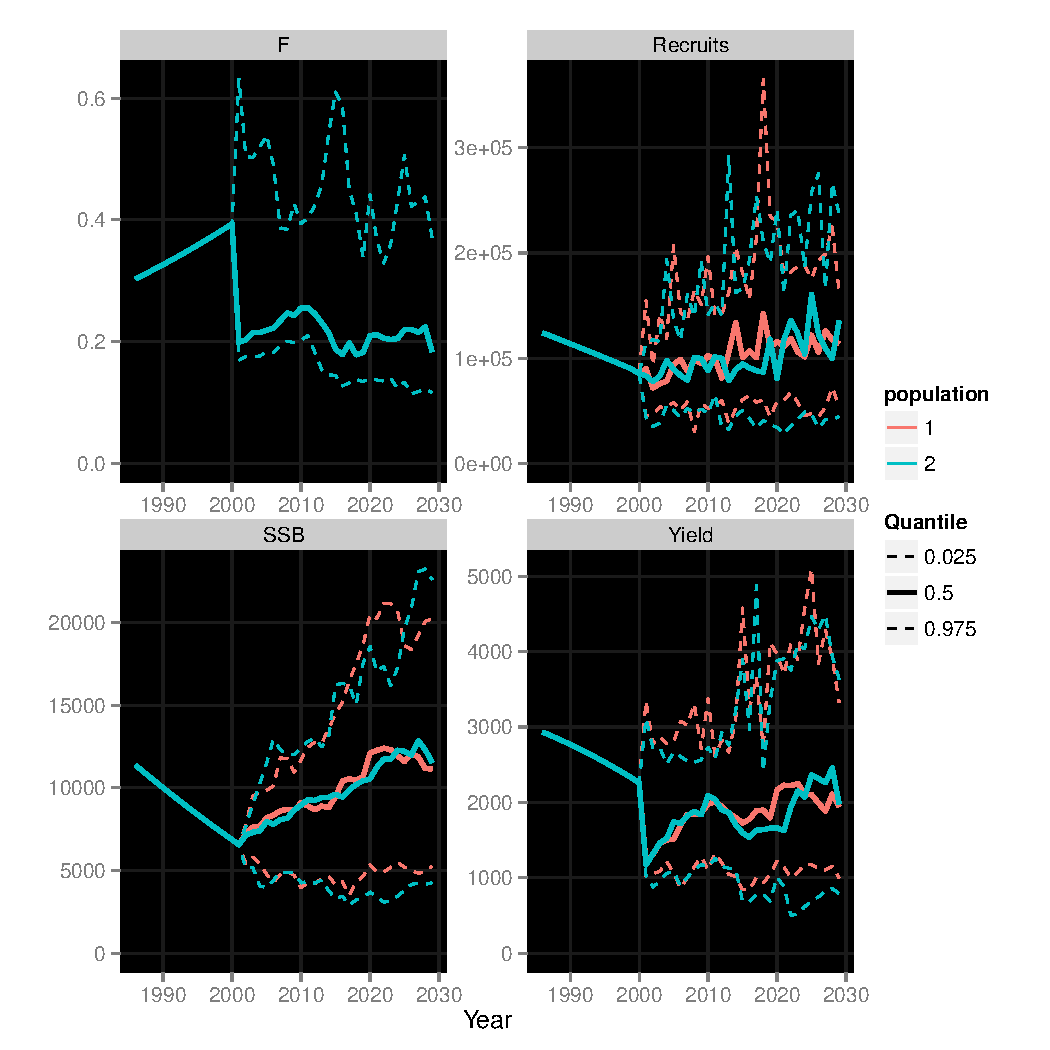
\includegraphics[width=.7\textwidth]{full-result1}
  \end{figure}
\end{frame}
\end{withoutheadline}

\begin{withoutheadline}
\begin{frame}{One full result}
  \begin{figure}
  \flushleft
  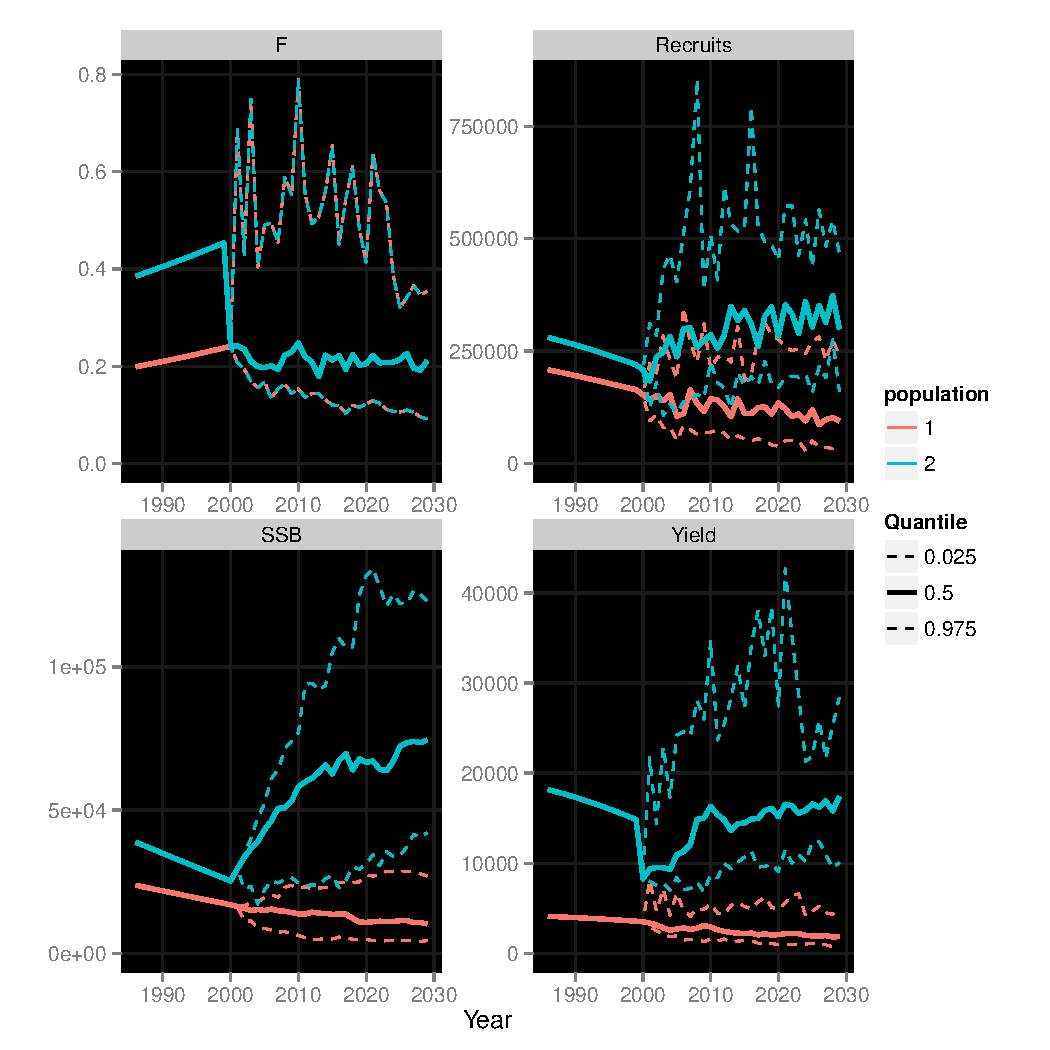
\includegraphics[width=.7\textwidth]{full-result2}
  \end{figure}
\end{frame}
\end{withoutheadline}

%%%%%%%%%%%%%%%%%%%%%%%%%%%%%%%%%%%%%%%%%%%%%

\begin{withoutheadline}
\begin{frame}{Results Summary}

\end{frame}
\end{withoutheadline}

%%%%%%%%%%%%%%%%%%%%%%%%%%%%%%%%%%%%%%%%%%%%%

\begin{frame}{Final Thoughts}
  \begin{itemize}
    \item Improve simulation speed by running in parallel on clusters
    \item Test other LH parameter sets
    \item Investigate link between virgin biomass and M etc.
    \item these is being explored at the ICES WGMG in two weeks  
  \end{itemize}
\end{frame}

%%%%%%%%%%%%%%%%%%%%%%%%%%%%%%%%%%%%%%%%%%%%%

\end{document}
